\documentclass{article}

\usepackage[utf8]{inputenc}
\usepackage{fullpage}
\usepackage{amsmath, amssymb, amsfonts, amsthm}
\usepackage{graphicx, subfig, float}
\usepackage{hyperref}
\usepackage{babel}

\parindent 0pt

\title
{
  Gags, gags, gags!!! \\
  \vspace{4pt}
  \normalsize
  \textit{Hierhin kommen alle Späße die uns einfallen!}
}
\author{}
\date{}

\begin{document}

\maketitle

\section{Fundamentals}

\href{https://knowyourphrase.com/how-do-you-like-them-apples}{Zitat} von \glqq Good Will Hunting\grqq: \\

Hunting: \glqq Do you like apples?\grqq

Rival: \glqq Yeah.\grqq

Hunting: \glqq Well, I got her number. How do you like them apples?\grqq

\begin{figure}[H]
\centering
\subfloat[Paul Winkler]{
  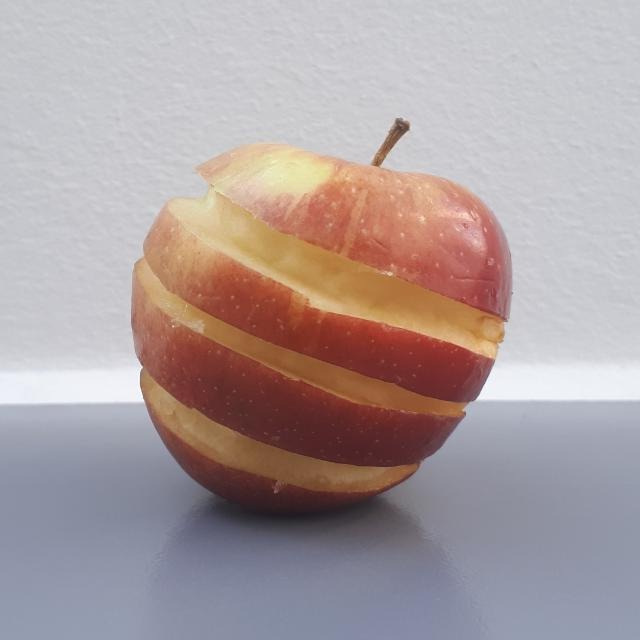
\includegraphics[width = 0.5 \textwidth]{images/apfel}
}
\subfloat[Michael Kaltenbäck]{
  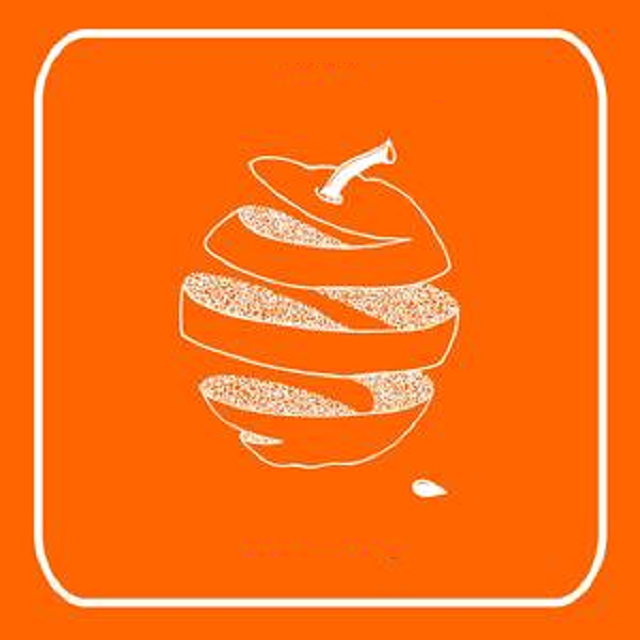
\includegraphics[width = 0.5 \textwidth]{images/apple}
}
\hspace{0mm}
\caption{Der (Bio-) Spindeltorus \textbf{Nicht Weglöschen!!!}}
\label{fig:apfel_apple}
\end{figure}

Ein \textit{Spindeltorus} entsteht durch Rotation des Kreissegmentes

\begin{align*}
  x = (R + r \cos{\theta}) \cos{\varphi} \\
  y = (R + r \cos{\theta}) \sin{\varphi} \\
  z = r \sin{\theta}
\end{align*}

um die $z$-Achse für $0 < R < r$, $R + r \cos{\theta} \geq 0$.

\section{Oberspaß}
\glqq Einheiz-Greis\grqq

\section{GIT}

\subsection{xkcd's}

\begin{figure}[h!]
  \centering
  
\includegraphics[width = 0.5 \linewidth]{images/git_2x.png}
\end{figure}

\subsection{Harry Potter}

\href{https://www.hp-lexicon.org/quote/professor-snape-ugly-git/}{Zitat} von \glqq Harry Potter and the Prisoner of Azkaban\grqq:\\

\glqq Mr. Prongs agrees with Mr. Moony, and would like to add that Professor Snape is an ugly git.\grqq

\section{Formulas}

\glqq A Kuh is a Vieh vom Mü-Viertl\grqq, d.h.

\begin{align}
  aq = a \phi \left( \frac{\mu}{4} \right)
\end{align}

\end{document}
